\section{Contraction of covariances}
\label{sec:contraction}
\motiv{To build a matrix product state on a chain, we join the virtual indices of on-site
tensors by maximally entangled pairs and then sum over them. For Gaussian
states the on-site tensors are covariances, the pairs are the bond covariance of
Definition~\ref{def:bond}, and the summation is one operation on matrices, the
contraction of Definition~\ref{def:contract}: it eliminates the labels of the joined
modes and returns a covariance on the labels that remain. The result is
admissible whenever the inputs are (Theorem~\ref{thm:contract}), so that a chain built by
repeated contraction is a covariance at every stage, and contracting two bonds through a
bond returns a bond (Theorem~\ref{thm:teleport}), which fixes the sign of the bond.
That the contraction is the covariance of the state obtained by projecting the
eliminated modes onto the pair is the fermionic linear-optics
calculus~\cite[Sec.~4]{bravyi}, \cite[Sec.~II]{ksvc}; Section~\ref{sec:gaussianmap} proves it on
Fock space (Theorem~\ref{thm:state-contract}).}

In this section we call a real matrix $\Gamma$ indexed by an
arbitrary finite set $I$ \emph{admissible} if $\Gamma^{\T}=-\Gamma$ and
$1-\Gamma^{\T}\Gamma\succeq0$, and \emph{pure} if $\Gamma^{\T}=-\Gamma$ and
$\Gamma^2=-1$; on the Majorana labels of $n$ modes these are the conditions of
Section~\ref{sec:majorana}, and the norm form of Theorem~\ref{thm:norm-form} holds for
every finite $I$ with the same proof. ``$M$ invertible'' means $\det M\neq0$, and
$M^{-1}$ is then the inverse matrix. For disjoint index sets $I_1,I_2$, $I_1\sqcup I_2$
is their union, and we write a matrix on $I_1\sqcup I_2$ in blocks with the $I_1$
labels first. The \emph{direct sum} of $\Gamma_1$ on $I_1$ and $\Gamma_2$ on $I_2$
is $\operatorname{diag}(\Gamma_1,\Gamma_2)$ on $I_1\sqcup I_2$, the matrix
$\Gamma_1\oplus\Gamma_2$ of Theorem~\ref{thm:sum} after grouping each system's labels
together. A set of modes $L$ carries the Majorana labels $x_a,y_a$ for $a\in L$,
written $x_L,y_L$ collectively; $1_L$ is the identity matrix indexed by $L$.

\subsection{The contraction and its admissibility}
Let $I=R\sqcup E$ be split into \emph{retained} and \emph{eliminated} labels (in the chains of
Section~\ref{sec:chain}: the physical and the virtual Majorana labels), and write
a matrix on $I$ in blocks
\[
 \Gamma=\begin{pmatrix}A&B\\C&D\end{pmatrix},\qquad
 A\in\R^{R\times R},\ B\in\R^{R\times E},\ C\in\R^{E\times R},\ D\in\R^{E\times E}.
\]
Let $\Gamma_p$ be a matrix on $E$, the \emph{pair covariance}.

\begin{definition}[Contraction]\label{def:contract}
If $1-D\Gamma_p$ is invertible,
\[
 \Gamma\star\Gamma_p=A+B\,\Gamma_p\,(1-D\Gamma_p)^{-1}C ,
\]
a matrix on $R$.
\end{definition}
\motiv{The formula is the Schur complement of the eliminated block of a $2\times2$
block system: if $(x,w)\mapsto(u,v)$ is the linear map $\Gamma$ and we impose $w=\Gamma_pv$
on the eliminated coordinates, then $u=(\Gamma\star\Gamma_p)x$
(displayed in the proof of Theorem~\ref{thm:contract}). The contraction preserves
admissibility because $\Gamma$ and $\Gamma_p$ are norm-nonincreasing (Theorem~\ref{thm:norm-form}),
hence so is $x\mapsto u$. For a pure $\Gamma_p$ the formula becomes
$A+B\,(D+\Gamma_p)^{-1}B^{\T}$ (Theorem~\ref{thm:pure-bond}), the form
of~\cite[Sec.~II]{ksvc}; the sign agrees with that reference once the pair is oriented as
in Definition~\ref{def:bond}, with $+1$ from the first copy to the second, and reversing the
orientation replaces $\Gamma_p$ by $-\Gamma_p$.}

\begin{lemma}[Push-through]\label{lem:push}
For square $X,Y$ of the same size, $\det(1-XY)=\det(1-YX)$, and if $1-XY$ is invertible
then $Y(1-XY)^{-1}=(1-YX)^{-1}Y$.
\end{lemma}
\begin{proof}
The determinant identity is Sylvester's: both sides equal the determinant of the block
matrix $\begin{pmatrix}1&X\\Y&1\end{pmatrix}$, obtained by eliminating either diagonal
block. From $Y(1-XY)=Y-YXY=(1-YX)Y$, multiply by $(1-YX)^{-1}$ on the left and
$(1-XY)^{-1}$ on the right.
\end{proof}

\begin{theorem}[Antisymmetry]\label{thm:antisym}
Let $\Gamma^{\T}=-\Gamma$, $\Gamma_p^{\T}=-\Gamma_p$, and $1-D\Gamma_p$ invertible. Then
$(\Gamma\star\Gamma_p)^{\T}=-\Gamma\star\Gamma_p$.
\end{theorem}
\begin{proof}
Antisymmetry of $\Gamma$ gives $A^{\T}=-A$, $D^{\T}=-D$ and $C=-B^{\T}$, so
$C^{\T}=-B$; antisymmetry of $\Gamma_p$ and $D$ gives
$(1-D\Gamma_p)^{\T}=1-\Gamma_p^{\T}D^{\T}=1-\Gamma_pD$. Then
\begin{align*}
 \bigl(B\Gamma_p(1-D\Gamma_p)^{-1}C\bigr)^{\T}
 &=C^{\T}\bigl((1-D\Gamma_p)^{\T}\bigr)^{-1}\Gamma_p^{\T}B^{\T}
 =(-B)(1-\Gamma_pD)^{-1}(-\Gamma_p)B^{\T}\\
 &=B\,(1-\Gamma_pD)^{-1}\Gamma_p\,B^{\T}
 =B\,\Gamma_p(1-D\Gamma_p)^{-1}B^{\T}
 =-B\,\Gamma_p(1-D\Gamma_p)^{-1}C ,
\end{align*}
using Lemma~\ref{lem:push} with $X=D$, $Y=\Gamma_p$ in the second line and then
$B^{\T}=-C$. So the second term changes sign under transposition, as does $A$.
\end{proof}

\begin{theorem}[Admissibility of the contraction]\label{thm:contract}
Let $\Gamma$ and $\Gamma_p$ be admissible and $1-D\Gamma_p$ invertible. Then
$\Gamma\star\Gamma_p$ is admissible.
\end{theorem}
\begin{proof}
Antisymmetry is Theorem~\ref{thm:antisym}; by the norm form it remains to show
$\|(\Gamma\star\Gamma_p)x\|\leq\|x\|$ for real $x\in\R^R$.
\begin{enumerate}
\item[(a)] Put
\[
 v=(1-D\Gamma_p)^{-1}Cx\in\R^E,\qquad w=\Gamma_pv\in\R^E,\qquad u=Ax+Bw\in\R^R .
\]
Then $u=(\Gamma\star\Gamma_p)x$ by definition, and $(1-D\Gamma_p)v=Cx$ gives
$v=Cx+Dw$. Hence
\[
 \Gamma\begin{pmatrix}x\\w\end{pmatrix}
 =\begin{pmatrix}Ax+Bw\\Cx+Dw\end{pmatrix}=\begin{pmatrix}u\\v\end{pmatrix}.
\]
\item[(b)] Admissibility of $\Gamma$ in norm form gives
$\|u\|^2+\|v\|^2\leq\|x\|^2+\|w\|^2$, and admissibility of $\Gamma_p$ gives
$\|w\|^2=\|\Gamma_pv\|^2\leq\|v\|^2$. Adding, $\|u\|^2\leq\|x\|^2$.
\end{enumerate}
\end{proof}
\begin{remark}\label{rem:invertibility}
Admissibility of $\Gamma$ and $\Gamma_p$ does not imply that $1-D\Gamma_p$ is
invertible: for $\Gamma=\begin{pmatrix}0&0\\0&D\end{pmatrix}$ with $D$ pure and
$\Gamma_p=-D$, $1-D\Gamma_p=1-1=0$. \motiv{For a pure pair covariance, Theorem~\ref{thm:pure-bond} turns the hypothesis into the
invertibility of $D+\Gamma_p$, which we check directly in each example.}
\end{remark}

\begin{theorem}[Pure pair covariances]\label{thm:pure-bond}
Let $\Gamma^{\T}=-\Gamma$ and let $\Gamma_p$ be pure. Then $1-D\Gamma_p$ is invertible
if and only if $D+\Gamma_p$ is, and in that case
\[
 \Gamma\star\Gamma_p=A+B\,(D+\Gamma_p)^{-1}B^{\T} .
\]
\end{theorem}
\begin{proof}
\begin{enumerate}
\item[(a)] Since $\Gamma_p^2=-1$, $\Gamma_p(-\Gamma_p)=1$, so $-\Gamma_p$ is invertible
with $(-\Gamma_p)^{-1}=\Gamma_p$, and
$(D+\Gamma_p)(-\Gamma_p)=-D\Gamma_p+1=1-D\Gamma_p$. Taking determinants, $\det(1-D\Gamma_p)$
and $\det(D+\Gamma_p)$ vanish together.
\item[(b)] When they do not vanish,
$(1-D\Gamma_p)^{-1}=(-\Gamma_p)^{-1}(D+\Gamma_p)^{-1}=\Gamma_p(D+\Gamma_p)^{-1}$, hence
$\Gamma_p(1-D\Gamma_p)^{-1}=\Gamma_p^2(D+\Gamma_p)^{-1}=-(D+\Gamma_p)^{-1}$ and, with
$C=-B^{\T}$, $B\Gamma_p(1-D\Gamma_p)^{-1}C=B(D+\Gamma_p)^{-1}B^{\T}$.
\end{enumerate}
\end{proof}
For a pair covariance that is not pure the two expressions differ \revs{in general}.

\subsection{The bond covariance and teleportation}
Let $L$ and $L'$ be two sets of modes matched by a bijection $a\mapsto a'$, with
Majorana labels $(x_L,x_{L'},y_L,y_{L'})$. In the chain of Section~\ref{sec:chain} the
first copy $L$ is the left virtual set of a site and the second copy $L'$ the right
virtual set of the previous site; we orient the bond from the first copy to the second,
$\beta_{x_ax_{a'}}=+1$.

\begin{definition}[Bond covariance]\label{def:bond}
The bond covariance on $L\sqcup L'$ is
\[
 \beta=\begin{pmatrix}J&0\\0&-J\end{pmatrix},\qquad
 J=\begin{pmatrix}0&1_L\\-1_L&0\end{pmatrix},
\]
where the outer blocks are the $x$ and $y$ labels and the inner blocks of $J$ are
$L$ and $L'$: $\beta_{x_ax_{a'}}=+1$, $\beta_{y_ay_{a'}}=-1$, all other entries zero.
\end{definition}
\motiv{For one pair of modes, $\beta$ has $\ii c_{x_a}c_{x_{a'}}$ and
$-\ii c_{y_a}c_{y_{a'}}$ both of expectation $1$; in the vacuum of
Corollary~\ref{cor:vacuum} the nonzero expectations are instead $\ii c_{x_a}c_{y_a}$
within one mode. The two-mode state with covariance $\beta$ is Theorem~\ref{thm:bondstate}.}

\begin{theorem}[Purity of the bond]\label{thm:bond-pure}
$\beta$ is pure.
\end{theorem}
\begin{proof}
$J^{\T}=-J$ and $J^2=-1$, so $\beta^{\T}=-\beta$ and
$\beta^2=\operatorname{diag}(J^2,J^2)=-1$.
\end{proof}

\begin{figure}[t]
\centering
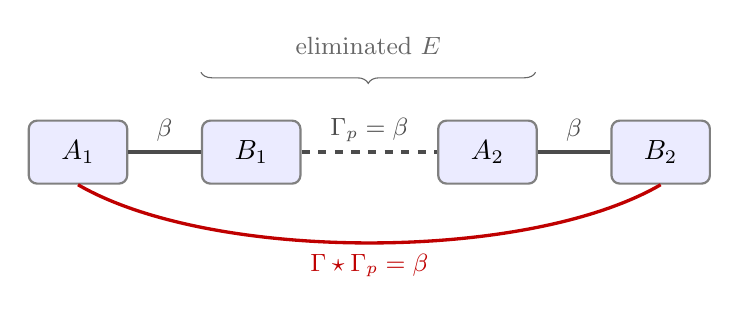
\begin{tikzpicture}[
  blk/.style={draw=black!50,fill=blue!8,thick,rounded corners=3pt,minimum width=1.25cm,minimum height=0.8cm},
  bond/.style={very thick,black!70},
  elim/.style={very thick,black!70,dashed},
  res/.style={very thick,red!75!black},
  lab/.style={font=\small}]
  \node[blk] (A1) at (0,0) {$A_1$};
  \node[blk] (B1) at (2.2,0) {$B_1$};
  \node[blk] (A2) at (5.2,0) {$A_2$};
  \node[blk] (B2) at (7.4,0) {$B_2$};
  \draw[bond] (A1) -- node[above,lab] {$\beta$} (B1);
  \draw[elim] (B1) -- node[above,lab] {$\Gamma_p=\beta$} (A2);
  \draw[bond] (A2) -- node[above,lab] {$\beta$} (B2);
  \draw[res] (A1.south) .. controls (1.7,-1.4) and (5.7,-1.4) .. node[below,lab] {$\Gamma\star\Gamma_p=\beta$} (B2.south);
  \draw[decorate,decoration={brace,amplitude=4pt,mirror},black!60] (B1.north west) ++(0,0.6) -- node[above=3pt,lab] {eliminated $E$} ++(4.25,0);
\end{tikzpicture}
\caption{Teleportation (Theorem~\ref{thm:teleport}). Each block is a copy of the
virtual label set $L$; solid lines are the bonds $\beta$ on $(A_1,B_1)$ and $(A_2,B_2)$,
the dashed line is the pair covariance $\Gamma_p=\beta$ on the eliminated labels
$E=B_1\sqcup A_2$. Contracting returns the bond $\beta$ on the retained pair $(A_1,B_2)$,
with the same sign and the same $x,y$ roles.}
\label{fig:teleport}
\end{figure}
\begin{theorem}[Teleportation]\label{thm:teleport}
Let two systems $I_1=A_1\sqcup B_1$ and $I_2=A_2\sqcup B_2$, each a matched pair of
copies of $L$, carry the bond covariance $\beta$ on $(A_1,B_1)$ and on $(A_2,B_2)$, and
let $\Gamma$ be their direct sum on $I_1\sqcup I_2$. Retain $R=A_1\sqcup B_2$,
eliminate $E=B_1\sqcup A_2$, and take $\Gamma_p=\beta$ on $(B_1,A_2)$. Then
$1-D\Gamma_p$ is invertible and $\Gamma\star\Gamma_p=\beta$ on $(A_1,B_2)$.
\end{theorem}
\begin{proof}
Neither bond has an entry within $A_1\sqcup B_2$ or within $B_1\sqcup A_2$, so $A=0$
and $D=0$; hence $1-D\Gamma_p=1$ is invertible and
$\Gamma\star\Gamma_p=B\Gamma_pC=-B\Gamma_pB^{\T}$. All matrices are block diagonal in the
$x$ and $y$ labels. In the $x$ sector the two bonds contribute $J$ on $(A_1,B_1)$ and on
$(A_2,B_2)$, so the retained--eliminated block is
\[
 B=\begin{array}{c|cc}
    & x_{B_1} & x_{A_2}\\ \hline
  x_{A_1} & 1_L & 0\\
  x_{B_2} & 0 & -1_L
 \end{array}
\]
and $\Gamma_p=J$ on $(B_1,A_2)$. Then
\[
 -BJB^{\T}
 =-\begin{pmatrix}1_L&0\\0&-1_L\end{pmatrix}\begin{pmatrix}0&1_L\\-1_L&0\end{pmatrix}\begin{pmatrix}1_L&0\\0&-1_L\end{pmatrix}
 =-\begin{pmatrix}0&-1_L\\1_L&0\end{pmatrix}=J
\]
on $(x_{A_1},x_{B_2})$. In the $y$ sector $B$ and $\Gamma_p$ both change sign, so
$-B\Gamma_pB^{\T}$ changes sign and equals $-J$ on $(y_{A_1},y_{B_2})$. Together,
$\Gamma\star\Gamma_p=\beta$ on $(A_1,B_2)$.
\end{proof}
Theorem~\ref{thm:teleport} (Figure~\ref{fig:teleport}) fixes the convention: with the bond of
Definition~\ref{def:bond} used both as the on-site resource and as the contracted pair,
contraction reproduces the bond without a change of sign or of the $x,y$ roles. Here
we orient the contracted pair from $B_1$ to $A_2$. The chain of Section~\ref{sec:chain}
orients its inter-site pairs the other way, from $A_{i+1}$ to $B_i$; since $A=0$ and $D=0$
here, the contraction is linear in $\Gamma_p$, and with the chain orientation the same
computation returns $-\beta$ on $(A_1,B_2)$, that is $\beta$ on $(B_2,A_1)$.
